\chapter{Gas de fermi de electrones libres} \label{Ch:06}

En este capítulo se comienza el estudio de los metales con un primer modelo en el que los electrones de valencia de los átomos del metal se \textit{independizan} cosntituyéndose en electrones de conducción que se mueven de una forma casi completamente libre a través del metal. De manera más precisa se supone que la red de iones positivos en el metal está inmóvil (red \textit{fría}) y además se sustituye por un fondo positivo de carga (a veces llamado \textit{modelo jalea}) de modo que el potencial eléctrico a que están sometidos los electrones de conducción es una constante que puede tomarse como cero. Se admite además que los electrones no interaccionan entre sí, pero debido a su carácter fermiónico les aplicaremos el Principio de Exclusión de Pauli. Hablaremos entonces de \textit{Gas de Fermi de elctrones libres}.

\section{Estados fundamentales del gas de Fermi}

\subsection{Niveles de energía}

Por tratarse de electrones independientes debemos calcular los niveles de un solo electrón, que luego serán ocupados por todos los electrones libres del metal: es la \textit{aproximación monoeléctrica}. Consideremos pues un electrón libre en un volumen $V=L_1L_2L_3$. La función de onda es, como es sabido, 

\begin{equation}
    \psi_\kn = V^{-1/2} e^{i \kn \cdot \rn} \label{Ec:06-01-01}
\end{equation}
con energía e impulso, respectivamente 

\begin{equation}
\begin{array}{ccc}
    \epsilon & = &\hbar^2 k^2 /2m \\
    \pn &= &  \hbar \kn
\end{array}
\end{equation}
Se aplican ahora a (\ref{Ec:06-01-01}) las condiciones de contorno periódicas:

\begin{equation}
    \begin{array}{ccc}
    \psi_\kn (x,y,z+L_3) & = & \psi_\kn (x,y,z) \\
    \psi_\kn (x,y+L_2,z) & = & \psi_\kn (x,y,z) \\
    \psi_\kn (x+L_1,y,z) & = & \psi_\kn (x,y,z) \\
    \end{array}
\end{equation}
que conducen a 
\begin{equation}
    k_i = n_i 2 \pi / L_i \quad (i=1,2,3 \ \text{y} \ n_i \in \mathbb{Z})
\end{equation}
De esta forma el volumen del espacio recíproca asociado a cada valor posible de $\kn$ es $8\pi^3 /V$, con densidad uniforme. Si ahora tenemos $N$ electrones para ``colocar'' el estado fundamental a $T=0$K consiste en ir llenando por energías crecientes los distintos estados monoelectrónicos respetando el Principio de Exclusión hasta agotar los $N$ electrones. La situación final es como se esquematiza en la figura \ref{Fig:06-01} (cada punto corresponde a dos electrones).

\begin{figure}[h!] \centering
    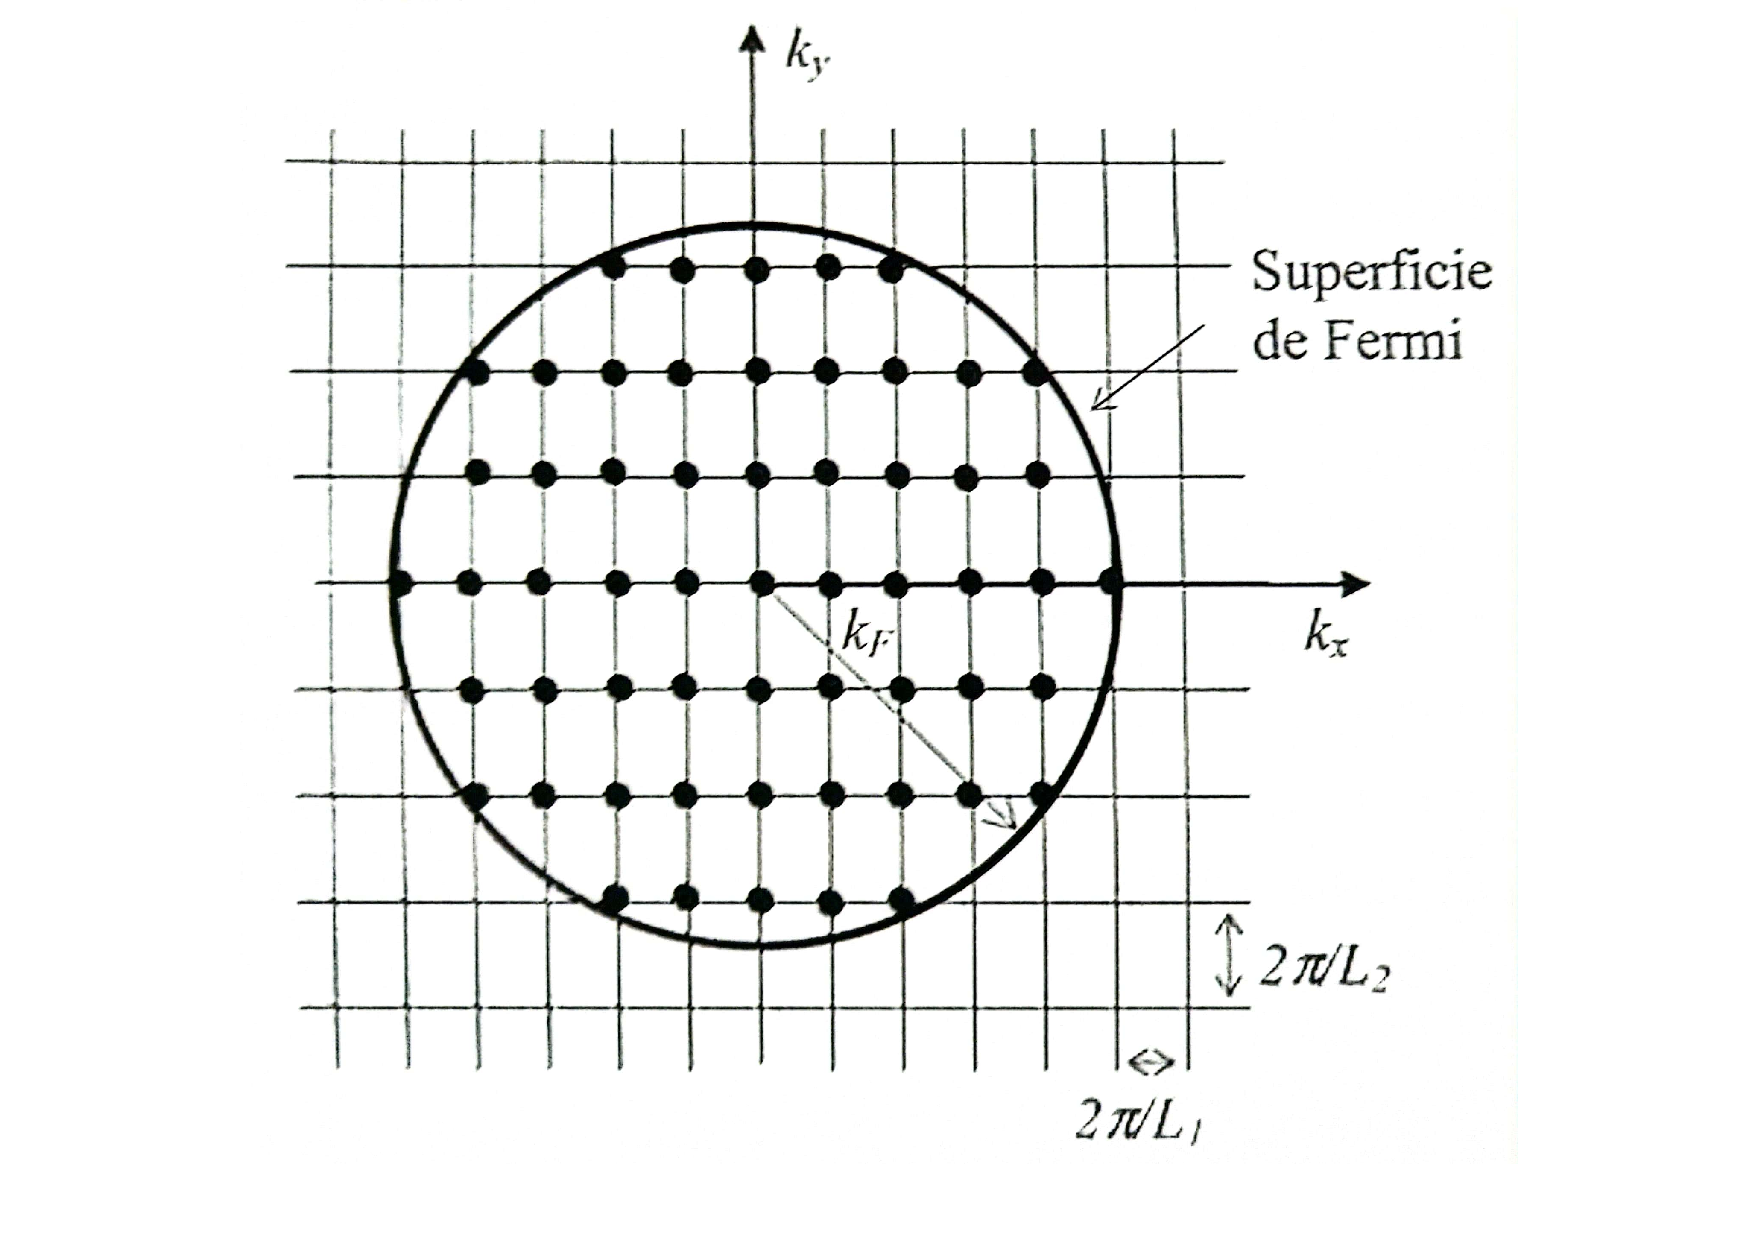
\includegraphics[scale=0.35]{Cuerpo/Ch_06/Fotos libro 1.pdf}
    \caption{Distribución de estados electrónicos ocupados en el espacio de fases.}
    \label{Fig:06-01}
\end{figure}    



La \textit{superficie de Fermi} es la superficie que separa los estados ocupados de los desocupados. A continuación vamos a definir los términos de Fermi:

\begin{itemize}
	\item \textbf{Vector de onda de Fermi (3D):}
	\begin{equation}
		k_F = (3\pi^2 n)^{1/3} \quad (n\equiv N/V) \label{Ec:06-01-05}
	\end{equation}
	\item \textbf{Vector de onda de Fermi (2D):}
	\begin{equation}
		k_F= \sqrt{2\pi n}
	\end{equation}
	\item \textbf{Energía de Fermi:}
	\begin{eqnarray}
		\varepsilon_F \equiv \frac{\hbar^2 k_F^2}{2m} \label{Ec:06-01-07}
	\end{eqnarray}
	\item \textbf{Velocidad de Fermi:}
	\begin{eqnarray}
	v_F \equiv \sqrt{2\varepsilon_F /m} \label{Ec:06-01-08}
	\end{eqnarray}
	\item \textbf{Temperatura de Fermi:}
	\begin{eqnarray}
		T_F \equiv k_B \varepsilon_F 
	\end{eqnarray}
\end{itemize}
Todos estos parámetros dependen sólo de la concentración electrónica $n$ uqe es conocida para metales: $10^{22}<n(\textbf{cm}^{-1})<10^{23}$. Numéricamente, resultan los siguientes valores:

\begin{equation*}
	\begin{array}{c}
	\varepsilon_F = 1-10 \unit{\eV} \\
	T_F = 10^4 - 10^5 \unit{K} \\
	v_F = (0.7-2)\times 10^8 \unit{\cm/s}\\
	v_F = (0.7-1.7)\times 10^8 \unit{\cm^{-1}}
	\end{array}
\end{equation*}
La \textbf{densidad de estados} $D(\varepsilon)$ se calculaa fácilmente haciendo referencia a la figura \ref{Fig:06-02}, resultando:

\begin{equation}
	D(\varepsilon) \D \varepsilon = 2 \times \frac{4\pi k^2 \D k}{8 \pi3 /V} = \frac{V}{2\pi2} \parentesis{\frac{2m}{\hbar2}}^{3/2} \sqrt{\varepsilon} \D \varepsilon \label{Ec:06-01-10}
\end{equation}
El factor $2$ da cuenta de los dos estados electrónicos posibles. Es útil expresar la densidad de estados $D(\varepsilon)$ en función de $\varepsilon_F$ combinando (\ref{Ec:06-01-10}), con (\ref{Ec:06-01-05}) y (\ref{Ec:06-01-07}) resulta:

\begin{equation}
	D(\varepsilon) = \frac{3}{2} \frac{N}{\varepsilon_F} \sqrt{\frac{\varepsilon}{\varepsilon_F}} \label{Ec:06-01-11}
\end{equation}	

A menudo es más útil trabajar con el número de estados por unidad de volumen del cristal, en cuyo caso basta hacer en (\ref{Ec:06-01-12}) la sustitución $N\rightarrow N/V=n$.
	
\begin{figure}[h!] \centering
    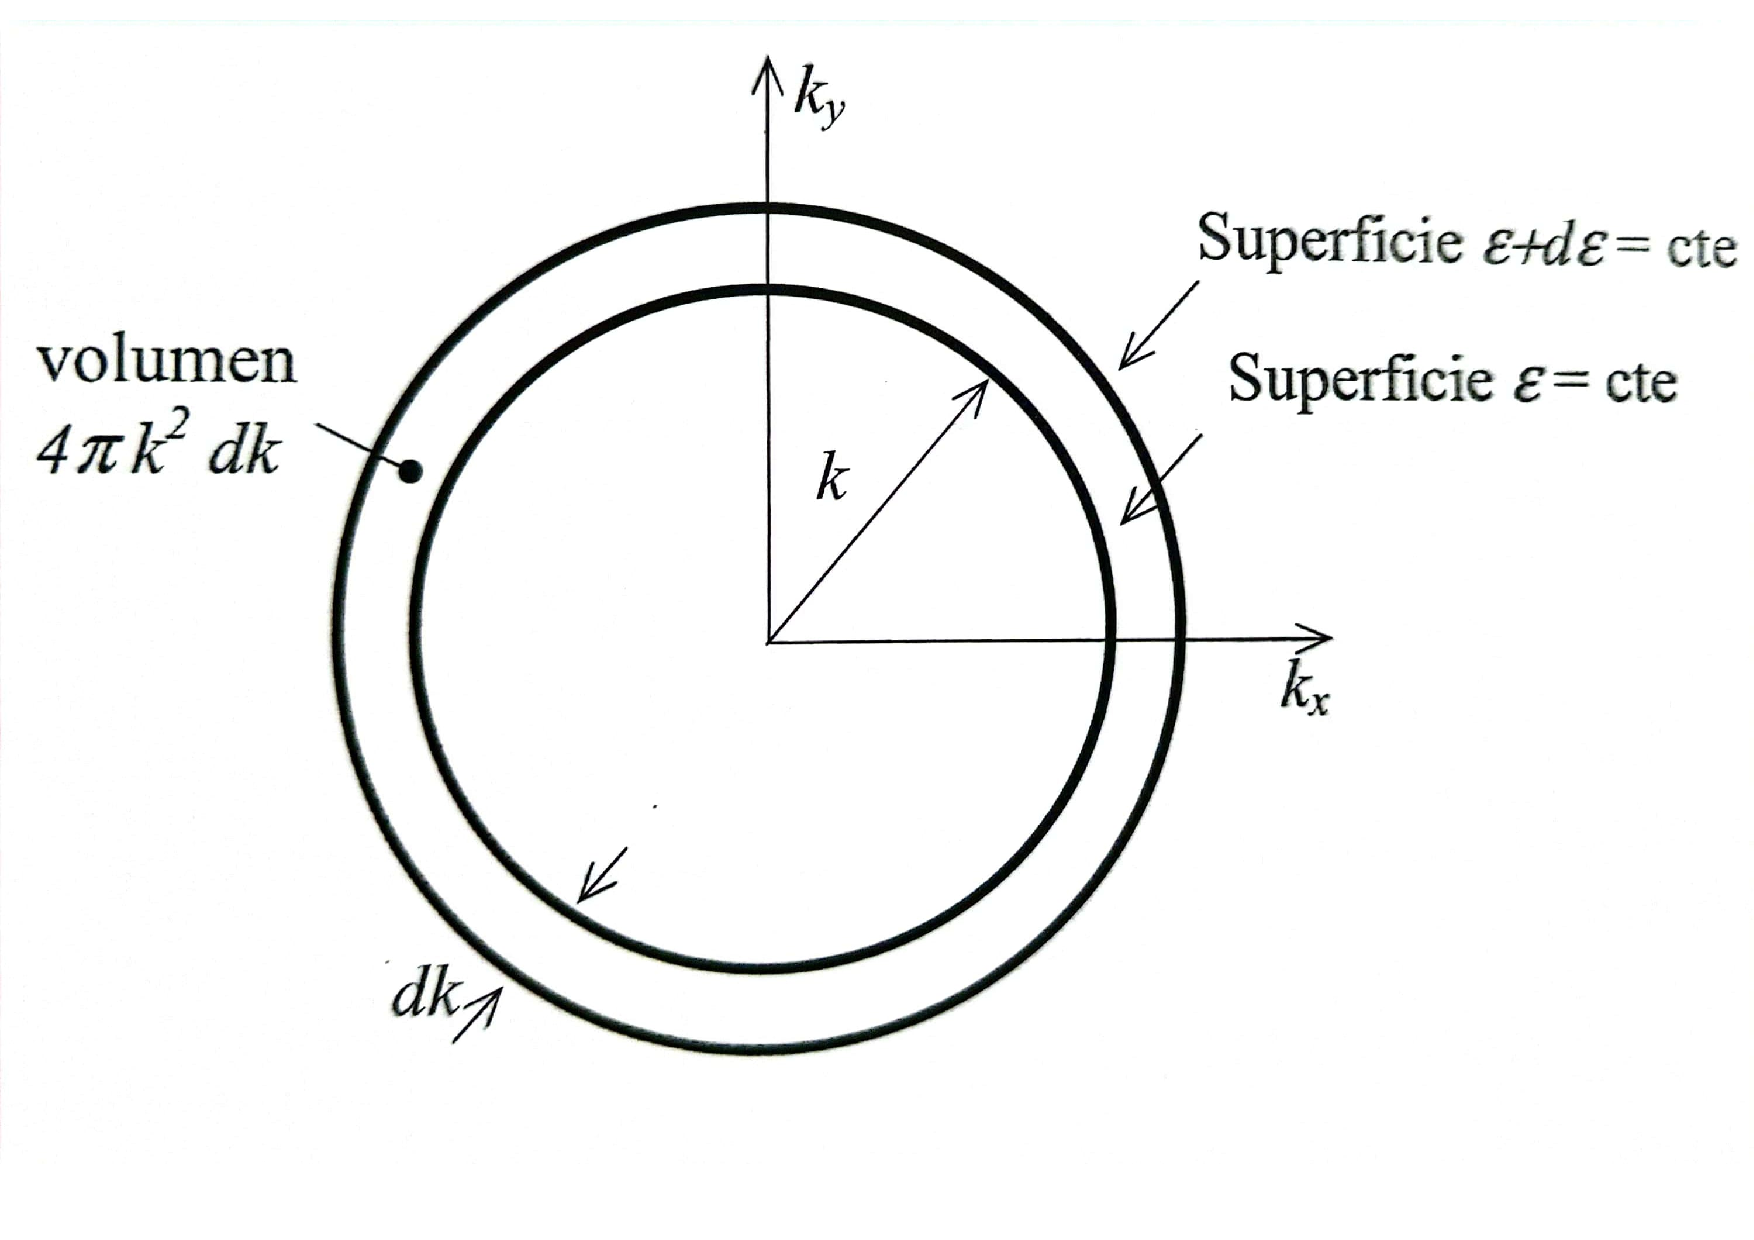
\includegraphics[scale=0.35]{Cuerpo/Ch_06/Fotos libro 2.pdf}
    \caption{Cálculo de la densidad de estados electrónicos.}
    \label{Fig:06-02}
\end{figure}  

\subsection{Ocupación de estados a $T>0$}

Se trata de saber cómo cambia el llenado de estados si el gas de electrones está a una temperatura finita. Por tratase de fermiones la respuesta la da la distribución de Fermi-Dirac, según la cual la probabilidad $f_{FD}$ de que un estado $\kn$ esté ocupado es:

\begin{equation}
	f_{FD} (\kn) = \frac{1}{e^{(\varepsilon(\kn)-\mu)/k_B T} +1}  \label{Ec:06-01-13}
\end{equation}
donde $\mu$ es el potencial química que verifica $f_{FD}(\mu)=1/2$. A $T=0$K, como esperaríamos, $f_{FD}(\varepsilon<\mu)=1$ y $f_{FD}(\varepsilon>\mu)=0$, por lo que podemos decir que $\varepsilon_F=\mu(T=0\textbf{K})$. A $T>0$ K la función $f_{FD}$ tiene el perfil que se grafíca en la figura \ref{Fig:06-03}. El potencial químico de la ligadura:

\begin{equation}
	N=\int_0^{\infty} f_{FD} (\varepsilon) D (\varepsilon) \D \varepsilon  \label{Ec:06-01-14}
\end{equation}
Al sustituir (\ref{Ec:06-01-11}) y (\ref{Ec:06-01-13}) en (\ref{Ec:06-01-14})  resulta una integral no analítica. Gracias a que $T\ll T_F$ las integrales de tipo (\ref{Ec:06-01-14}) se pueden aproximar por la llamada \textit{expansión de Sommerfeld} 

\begin{eqnarray}
	\int_{0}^{\infty} H(\varepsilon) f_{FD} (\varepsilon)  \D \varepsilon \approx \int_0^\mu H(\varepsilon) \D \varepsilon + \frac{\pi2 k_B^2 T^2}{6} \derivadas{\D H}{\D \varepsilon} (\mu)
\end{eqnarray}
Aplicando esta relación a (\ref{Ec:06-01-14}), tras alguna manipulación se llega a 

\begin{equation}
	\mu (T) = \mu(0) \ccorchetes{1-\frac{1}{3} \parentesis{\frac{\pi T}{2 T_F}}^2}
	\label{Ec:06-01-15}
\end{equation}
Usando los valores característicos para $T_F$, la lectura  de (\ref{Ec:06-01-15}) es que para que metales, incluso a la temperatura ambiente, se puede aproximar $\mu (T) \approx \varepsilon_F$ dentro del $0.01\%$, y concluimos que el gas electrónico resulta sólo muy ligeramente alterado de $T=0$ K a $T\sim 300$ K. Por tanto, en muchos casos se podrá aproximar la energía total a cualquier temperatura:

\begin{equation}
	U(T) = \int_0^\infty \varepsilon D(\varepsilon) f_{FD} \D \varepsilon 
\end{equation}
por la correspondiente a $T=0$ K (energía del punto cero):

\begin{equation}
	U(0) = \int_0^{\varepsilon_F} \varepsilon D(\varepsilon) \D \varepsilon
\end{equation}
pues $f_{FD}(\varepsilon,T)=1$ para $\varepsilon\leq\varepsilon_F$ y $f_{FD} (\varDelta,T)=0$ para $\varepsilon>\varepsilon_F$. Si sustituimos (\ref{Ec:06-01-11})	en la anterior expresión e integramos se obtiene:

\begin{equation}
	U(0)=\frac{3}{5} N \varepsilon_F
\end{equation}
de modo que la energía por electrón es, por (\ref{Ec:06-01-07}):

\begin{equation}
	u(0)=\frac{3}{5} \varepsilon_F = \frac{3}{5} \parentesis{\frac{\hbar^2 k_F^2}{2m}} = \frac{3\hbar^2}{10m} (3 \pi^2 n)^{2/3}
\end{equation}
que es la energía que fue utilizada al tratar el enlace metálico.


\begin{figure}[h!] \centering
    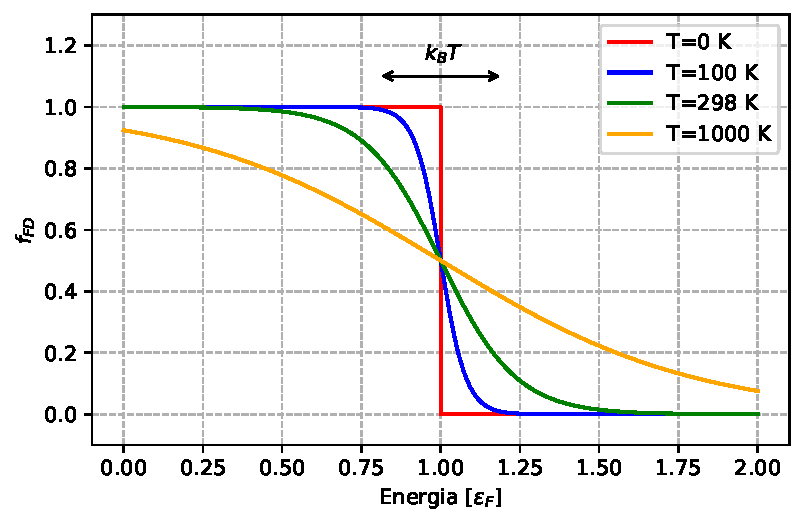
\includegraphics[scale=0.75]{Cuerpo/Ch_06/06-Fermi-Dirac.pdf}
    \caption{Distribución de Fermi-Dirac.}
    \label{Fig:06-03}
\end{figure}    

\subsection{Interacción electrón-electrón}

Es un metal la distancia media entre electrones de conducción es del orden de unos pocos $\unit{\angstrom}$ y, sin embargo, los recorridos libres medios para las colisiones elcetrón-electrón son mayores que $10^4 \unit{\angstrom}$ a temperatura ambiente, y superiores a 10 cm a 1 K. Uno de los factores responsables de esta falta de interacción entre electrones y que justifica la aproximación de electrones independientes es el Principio de Exclusión.

\begin{figure}[h!] \centering
    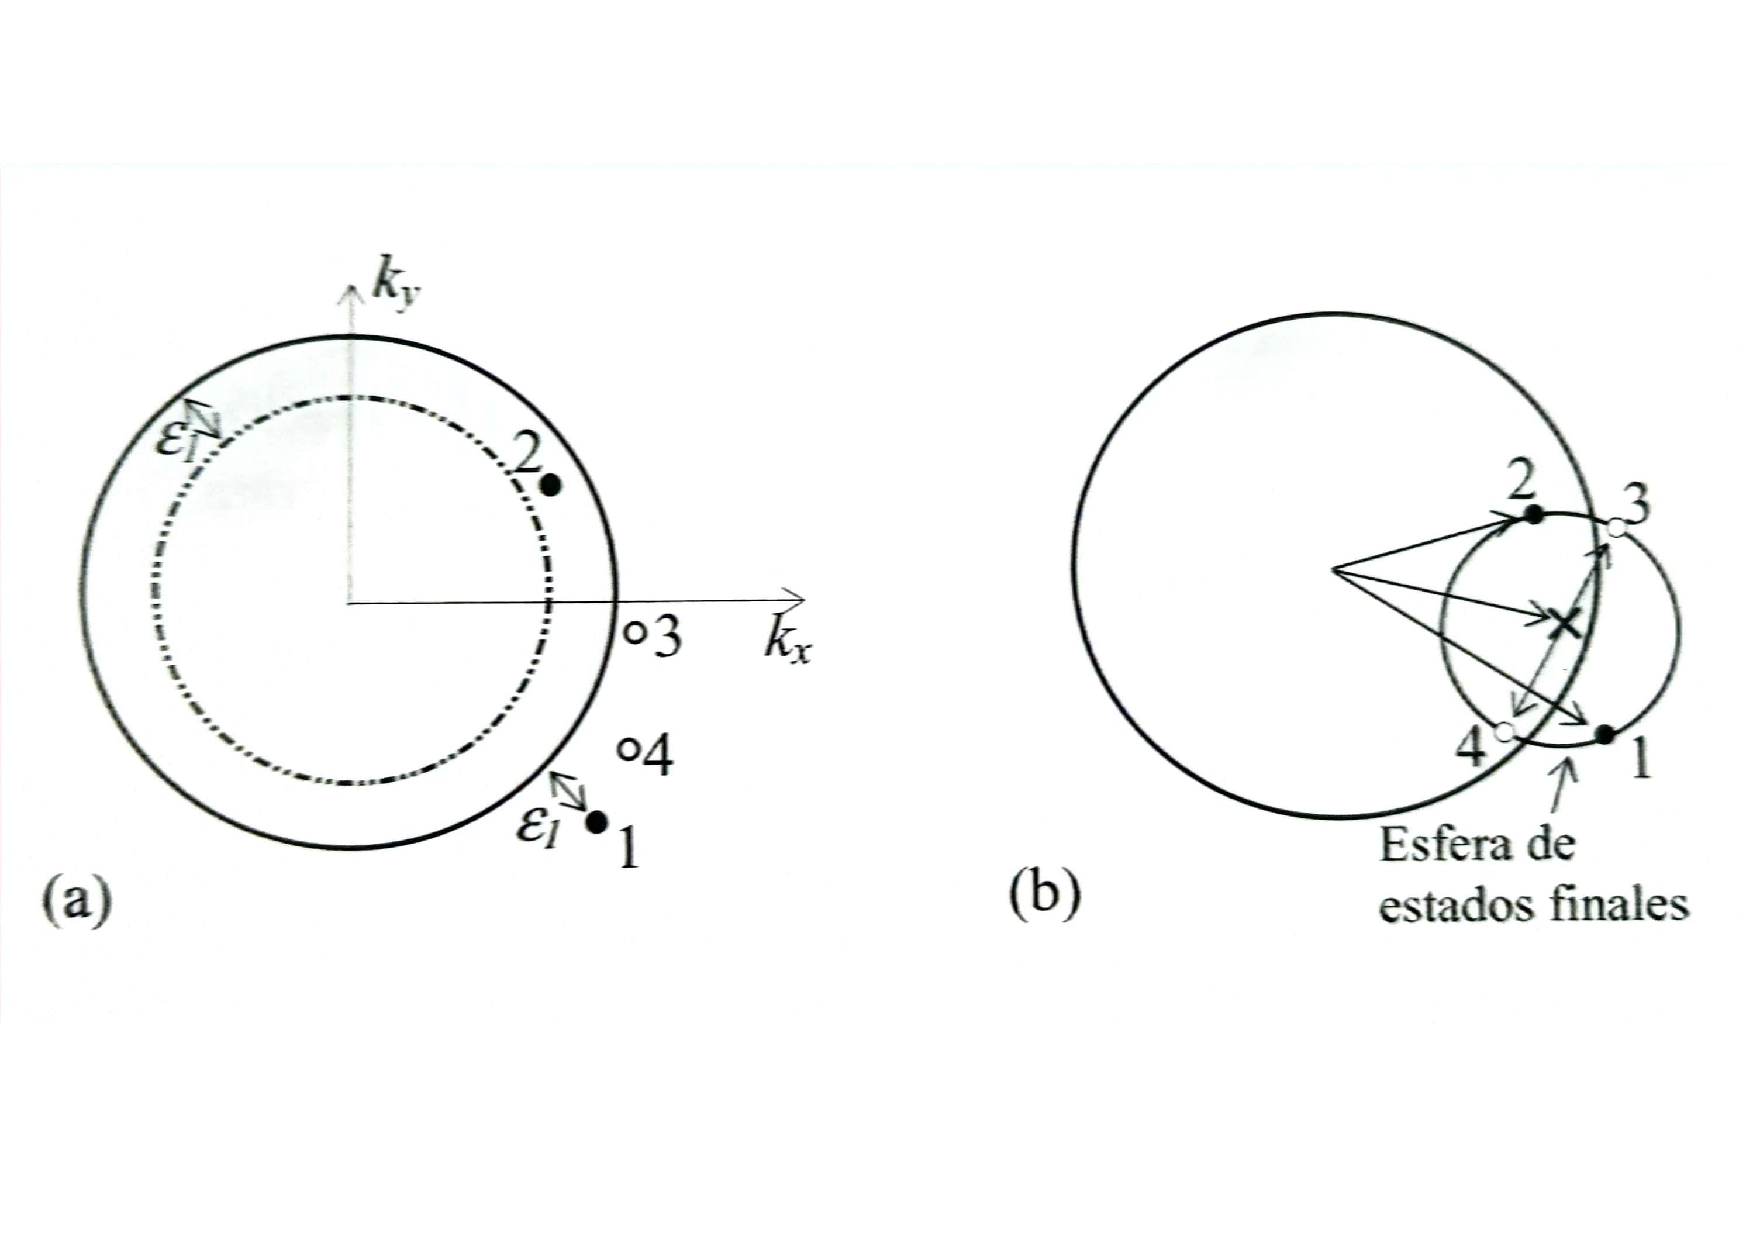
\includegraphics[scale=0.35]{Cuerpo/Ch_06/Fotos libro 4.pdf}
    \caption{Restricción a los procesos de colisión $e^- - e^-$ debido a las leyes de conservación de la energía (a) y del momento (b).}
    \label{Fig:06-04}
\end{figure}  

Consideremos la situación especialmente sencilla de una esfera de Fermi con un solo electrón excitado 1 con energía $\varepsilon_1$ respecto del nivel de Fermi. Como ilustra la figura \ref{Fig:06-04} (a), no todos los electrones 2 pueden colisionar con el 1, de modo que $1+2\rightarrow3+4$, pues los estados finales 3 y 4 deben estar desocupados. La condición $\varepsilon_3 + \varepsilon_4 = \varepsilon_1 + \varepsilon_2$ exige $|\varepsilon_2|<\varepsilon_1$ por lo que sólo una fracción $\sim \varepsilon_1 / \varepsilon_F$ de los electrones totales constituye un blanco para el electrón 1. La condición $\kn_1 + \kn_2 = \kn_3 + \kn_4$ limita aún más los estados finales: deben caer en la esfera de estados finales que ilustra la figura \ref{Fig:06-04} (b), y fuera del mar de Fermi la fracción permitida resulta ser también $\sim \varepsilon_1 / \varepsilon_F$. El producto de las dos fracciones es $\sim (\varepsilon_1/\varepsilon_F)^2$. 
En presencia de una temperatura finita puede equipararse $\varepsilon_1$ con $k_BT$, con lo que el Principio de Exclusión reduce las colisiones electrón-electrón en un factor $\sim (k_BT/\varepsilon_F)^2 \sim 10^4$. El correspondiente recorrido libre a temperatura ambiente es $\sim 10^4 \ \unit{\angstrom}$, mucho mayor que el debido a la interacción electrón-fonón.

\section{Capacidad térmica electrónica}

La contribución electrónica a la capacidad térmica medida en metales es $\sim 1\%$. Si los electrones fueran partículas clásicas la capacidad debería ser $\frac{3}{2} N k_BT$ y la energía que ganan $\sim k_B T$. Así pues $U(T) \approx U(0)+\frac{3N}{2\varepsilon_F} k_B^2 T^2$ y entonces

\begin{eqnarray}
	C_{el} \approx 3 N k_B \frac{T}{T_F}
\end{eqnarray}
que es directamente proporcional a $T$, de acuerdo con los resultados experimentales, y mucho menor que el valor clásico $\frac{3}{2} Nk_B$  debido a que $T\ll T_F$. El cálculo más formal se realiza a partir de $U=\int_{0}^{\infty} \varepsilon D(\varepsilon) f_{FD} (\varepsilon) \D \varepsilon$ que, vía la expansión de Sommerfeld, conduce a 

\begin{eqnarray}
	C_{el} = \frac{\pi^2}{2} N k_B \frac{T}{T_F}  \label{Ec:06-02-02}
\end{eqnarray}
La medida de la capacidad térmica electrónica debe hacerse a muy bajas temperaturas para no ser enmascarada por la contribución de la red (que es proporcional a $T^3$ cuando $T\rightarrow 0$). La dependencia lineal con $T$ se verifica excelentemente, pero de acuerdo del coeficiente $\gamma$ en $c_{el} = \gamma T$ es, como ilustra la tabla \ref{Tab:06-01}, muy variable y en algunos casos muy alejado del valor experimental.

\begin{table}[h!] \centering
	\begin{tabular}{cccc} 
		Elemento & $\gamma_{\text{el.libres}}$ &  $\gamma_{\text{exp}}$ & cociente \\
 		& ($10^{-4} \frac{\text{cal}}{\text{mol}\cdot\text{K}^2}$) & ($10^{-4} \frac{\text{cal}}{\text{mol}\cdot\text{K}^2}$)  &  \\ \hline
 		Li & 1.8 & 4.2 & 2.3 \\
 		Na & 2.6 & 3.5 & 1.3 \\
 		Cs & 5.3 & 7.7 & 1.5 \\
 		Cu & 1.2 & 1.6 & 1.3 \\
 		Au & 1.5 & 1.6 & 1.1 \\
 		Sr & 4.3 & 8.7 & 2.0 \\
 		Fe & 1.5 & 12 & 8.0 \\
 		Zn & 1.8 & 1.4 & 0.78 \\
 		Pb & 3.6 & 7.0 & 1.9 \\
 		Bi & 4.3 & 0.2 & 0.047 
	\end{tabular}	
	\caption{Predicción de la teoría de $e^-$ libres y resultado experimental para el coeficiente $\gamma$ de distintos elementos.}
	\label{Tab:06-01}
\end{table}

\section{Conductividad eléctrica DC}
\subsection{Modelo cinético de Drude y ecuación dinámica}

Los otros metales se caracterizan por una alta conductividad eléctrica, $\sigma$, comparada con otros materiales [$10^8$-$10^7$ ($\Omega$m)$^{-1}$ frente a $10^5$-$10^{-4}$ ($\Omega$m)$^{-1}$ en semiconductores y hasta $10^{-16}$ ($\Omega$m)$^{-1}$ en aislantes]. Electrones completamente libres e independientes (es decir, no interaccionantes con la red o entre ellos) darían lugar a una conductividad eléctrica infinita. Se introduce por tanto un modelo cinético similar al utilizado en el capítulo \ref{Ch:05} con fonones, según el cual los electrones colisionan con una probabilidad de tiempo $\tau^{-1}$ con fonones, defectos reticulares y en menor medida con otros electrones (\textit{modelo de Drude}). En este modelo cinético los electrones se tratan clásicamente. Esto es posible porque podemos formar, a partir de las funciones de onda (\ref{Ec:06-01-01}), un paquete de ondas de extensión espacial $\Delta x$ verificando $\Delta k \Delta x \sim 1$. Como $\Delta k$ debe estar bien definido, es decir $\Delta k \ll k_F \sim a^{-1}$, debe ser $\Delta x \gg a$. Por tanto, el modelo será aplicable siempre que las características de posibles perturbaciones (la longitud de onda de campos aplicados o el recorrido libre medio, ver más abajo) sean mucho mayores que $a$. 

Para obtener una ecuación dinámica para los electrones colisionantes, supongamos que $\pn(t)= m \vn(t)$ es el impulso medio de la colectividad de electrones y $\fn(t)$ la fuerza media. Si se sigue la evolución del gas de $t$ a $t+\D t$ se tiene:

\begin{equation}
	\pn (t+\D t) = \parentesis{1-\frac{\D t}{\tau}} \ccorchetes{\pn(t)+\fn(t)\D t} + o(\D t^2)
\end{equation}
donde se ha restado el impulso de las $\D t/\tau$ partículas que han colisionado en el intervalo $\D t$. Teniendo en cuenta que $\pn(t+\D t)=\pn(t)+(\D \pn / \D t)\D t$, la relación anterior conduce inmediatamente a 

\begin{equation}
	\derivadas{\pn(t)}{t} \equiv - \frac{\pn(t)}{\tau} +  \fn(t) \label{Ec:06-03-02}
\end{equation}



\subsection{Ley de Ohm}
Bajo la aplicación de un campo eléctrico se tiene que $\fn = \En$. En régimen estacionario $(\D \pn / \D t = 0)$, por (\ref{Ec:06-03-02}) cada electrón gana un impulso de $\delta \pn = -er\Encal$ ($\Encal$ es el campo eléctrico). Podemos decir que la esfera de Fermi se desplaza globalmente un vector de onda $\delta k = -er\Encal /\hbar$ (obsérvese figura \ref{Fig:06-05}). obsérvese que la pequeñez de $\tau$ hace que $\delta k \ll k_F$. La densidad de corriente eléctrica asociada a dicho desplazamiento es $$\jn=n(-e)\vn=-(ne/m)\delta \pn = (ne^2 r/m)\Encal$$  Este modelo predice por tanto la relación lineal $\jn=\sigma \Encal$ que es precisamente la \textbf{Ley de Ohm}. La constante de proporcionalidad (\textit{conductividad eléctrica}) se expresa en el marco de este modelo según:

\begin{eqnarray}
	\sigma = \frac{ne^2\tau}{m} \label{Ec:06-03-03}
\end{eqnarray}
La dificultad de la verificación de (\ref{Ec:06-03-03}) es que $\tau$ no es, en principio, conocido. Lo único que podemos decir es que identificando $\sigma$ en (\ref{Ec:06-03-03}) con valores experimentales resulta $\tau(300\unit{K})\sim10^{-14}\unit{s}$, lo que corresponde a un recorrido libre medio $\ell = v_F \tau$ de $\sim 100 \unit{\angstrom}$

\begin{figure}[h!] \centering
    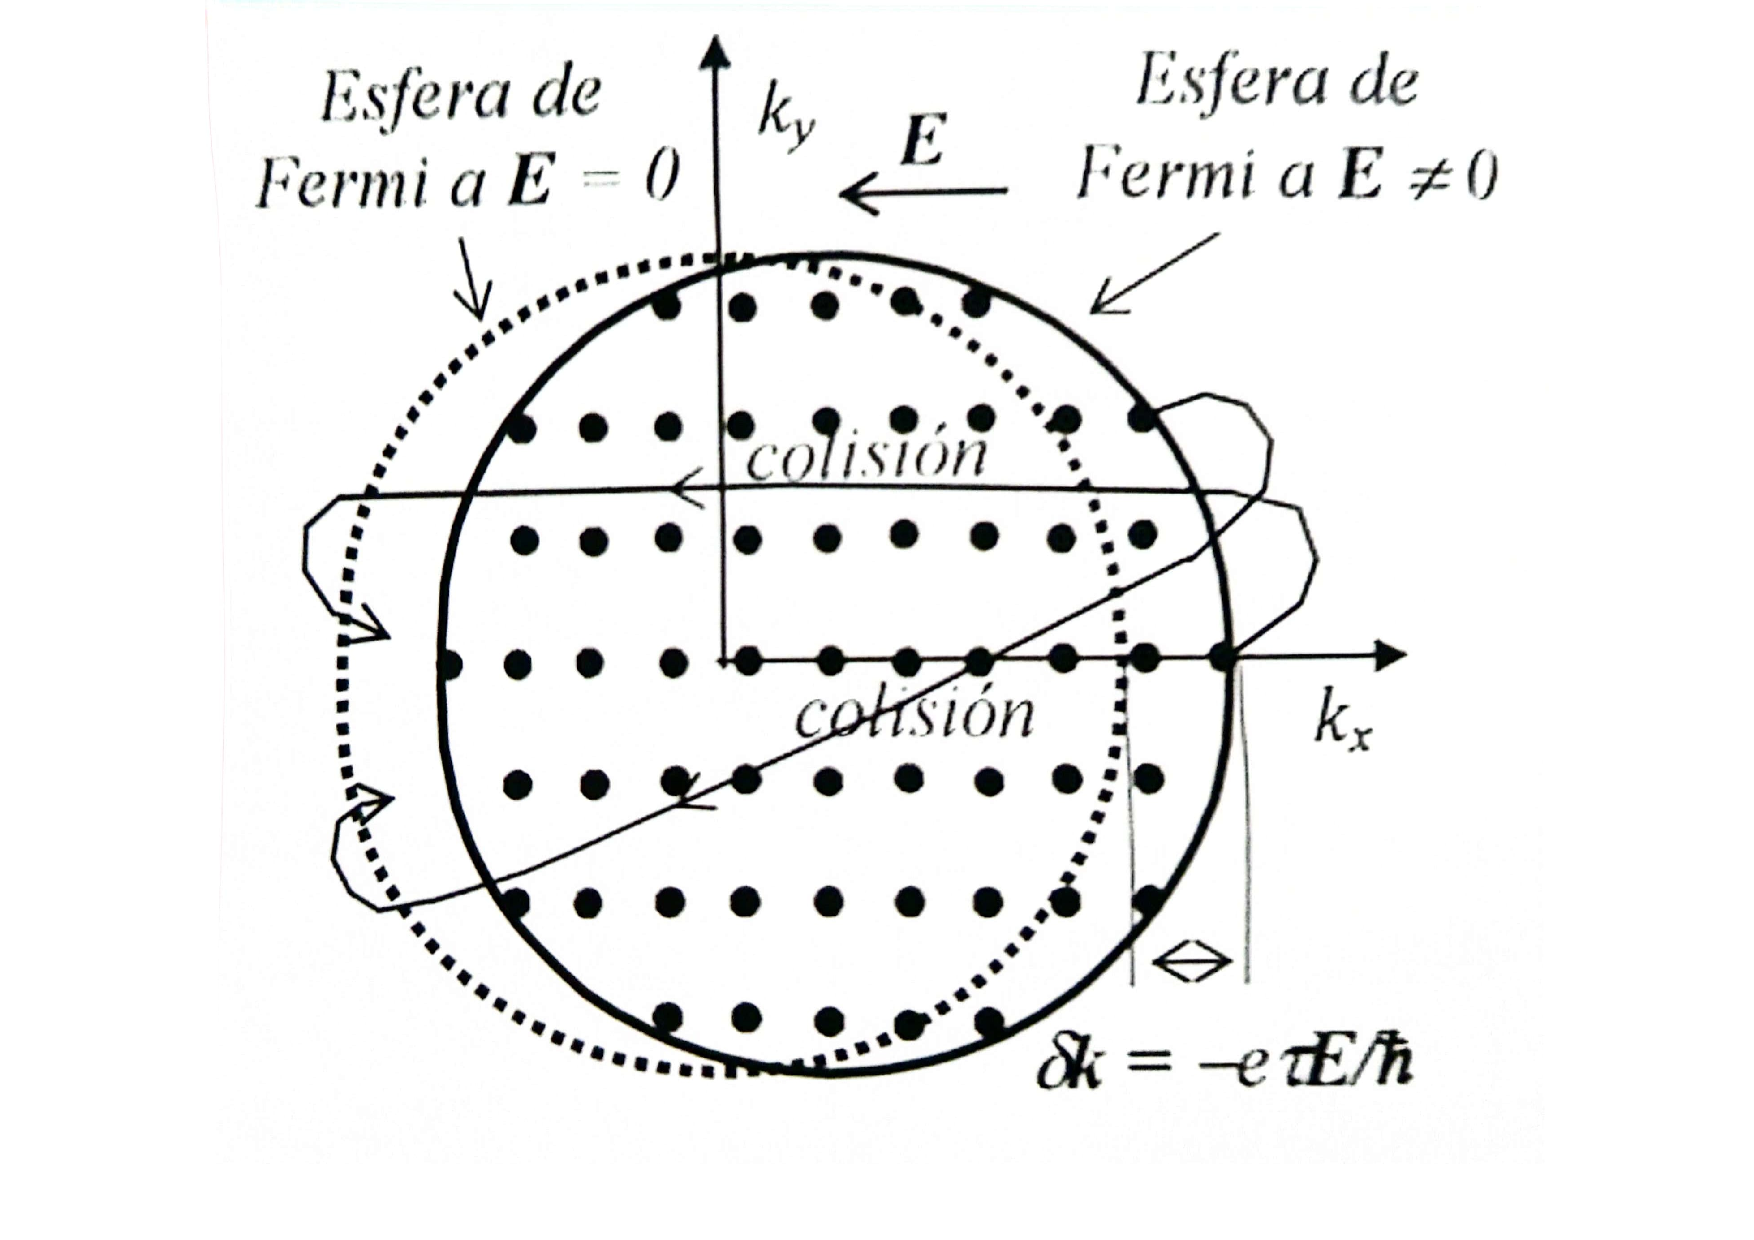
\includegraphics[scale=0.35]{Cuerpo/Ch_06/Fotos libro 5.pdf}
    \caption{Desplazamiento de la ``esfera de Fermi'' bajo la aplicación de un campo eléctrico. Las líneas indican algunos procesos de colisión permitidos.}
    \label{Fig:06-05}
\end{figure}  

\subsection{Dependencia con la temperatura de la conductividad eléctrica}

Si admitimos que los dos mecanismmos de scattering principales (fonones y defectos) son independientes entre sí, la probabilidad de colisión por unidad de tiempo $\tau^{-1}$ será la suma de las debidas a ambos mecanismos por separado:

\begin{eqnarray}
	\tau^{-1} = \tau_{\text{def}}^{-1} +\tau_{\text{fon}}^{-1}
    \label{Ec:06-03-04}
\end{eqnarray}
Como los defectos estructurales en un cristal (impurezas qímicas, microgrietas, dislocaciones, etc.) no cambian esencialmente con la temperatura, dan una contribución a $\sigma$ constante. En cuanto a los fonones, la probabilidad de colisión variará porque, en particular, varía el número de aquellos. Si combinamos (\ref{Fig:06-04}) y (\ref{Fig:06-05}) tenemos que para la resisitividad eléctrica $\rho\equiv 1/\sigma=m/ne^2 \tau$:

\begin{eqnarray}
	\rho = \rho_{\text{def}} + \rho_{\text{fon}} (T)
\end{eqnarray}
resultado que se conoce como la \textit{regla de Matthiesen}. A bajas temperaturas se tiene $\rho\approx \rho_{\text{def}}$, pues $\rho_{\text{fon}}(T)\rightarrow0$ al no existir fonones. En cristales ultrapuros y a muy bajas temperaturas $\tau$ o $\ell$ (y por tanto $\sigma$) pueden llegar a ser hasta 6 órdenes de magnitud mayores que a temperatura ambiente. A altas temperaturas, en el límite clásico ($T>\theta_{\text{Debye}}$) la distribución energética de los fonones cambia poco y lo que cuenta es su número medio. En particular , cabe esperar $\tau \propto \langle n \rangle_{\text{fon}}^{-1}$ y por tanto $\rho \propto \langle n \rangle_\text{fon}$. Como $\langle n \rangle_\text{fon} \propto T$ se predice la dependencia lineal de $\rho$ con $T$. Esto es en efecto lo que se encuentra experimentalmente en metales (figura \ref{Fig:06-06}). En el caso de medios desordenados como aleaciones, metales amorfos, etc. predomina la dispersión electrónica por defectos sobre la dispersión por fonones y $\rho$ es casi constante.

\begin{figure}[h!] \centering
    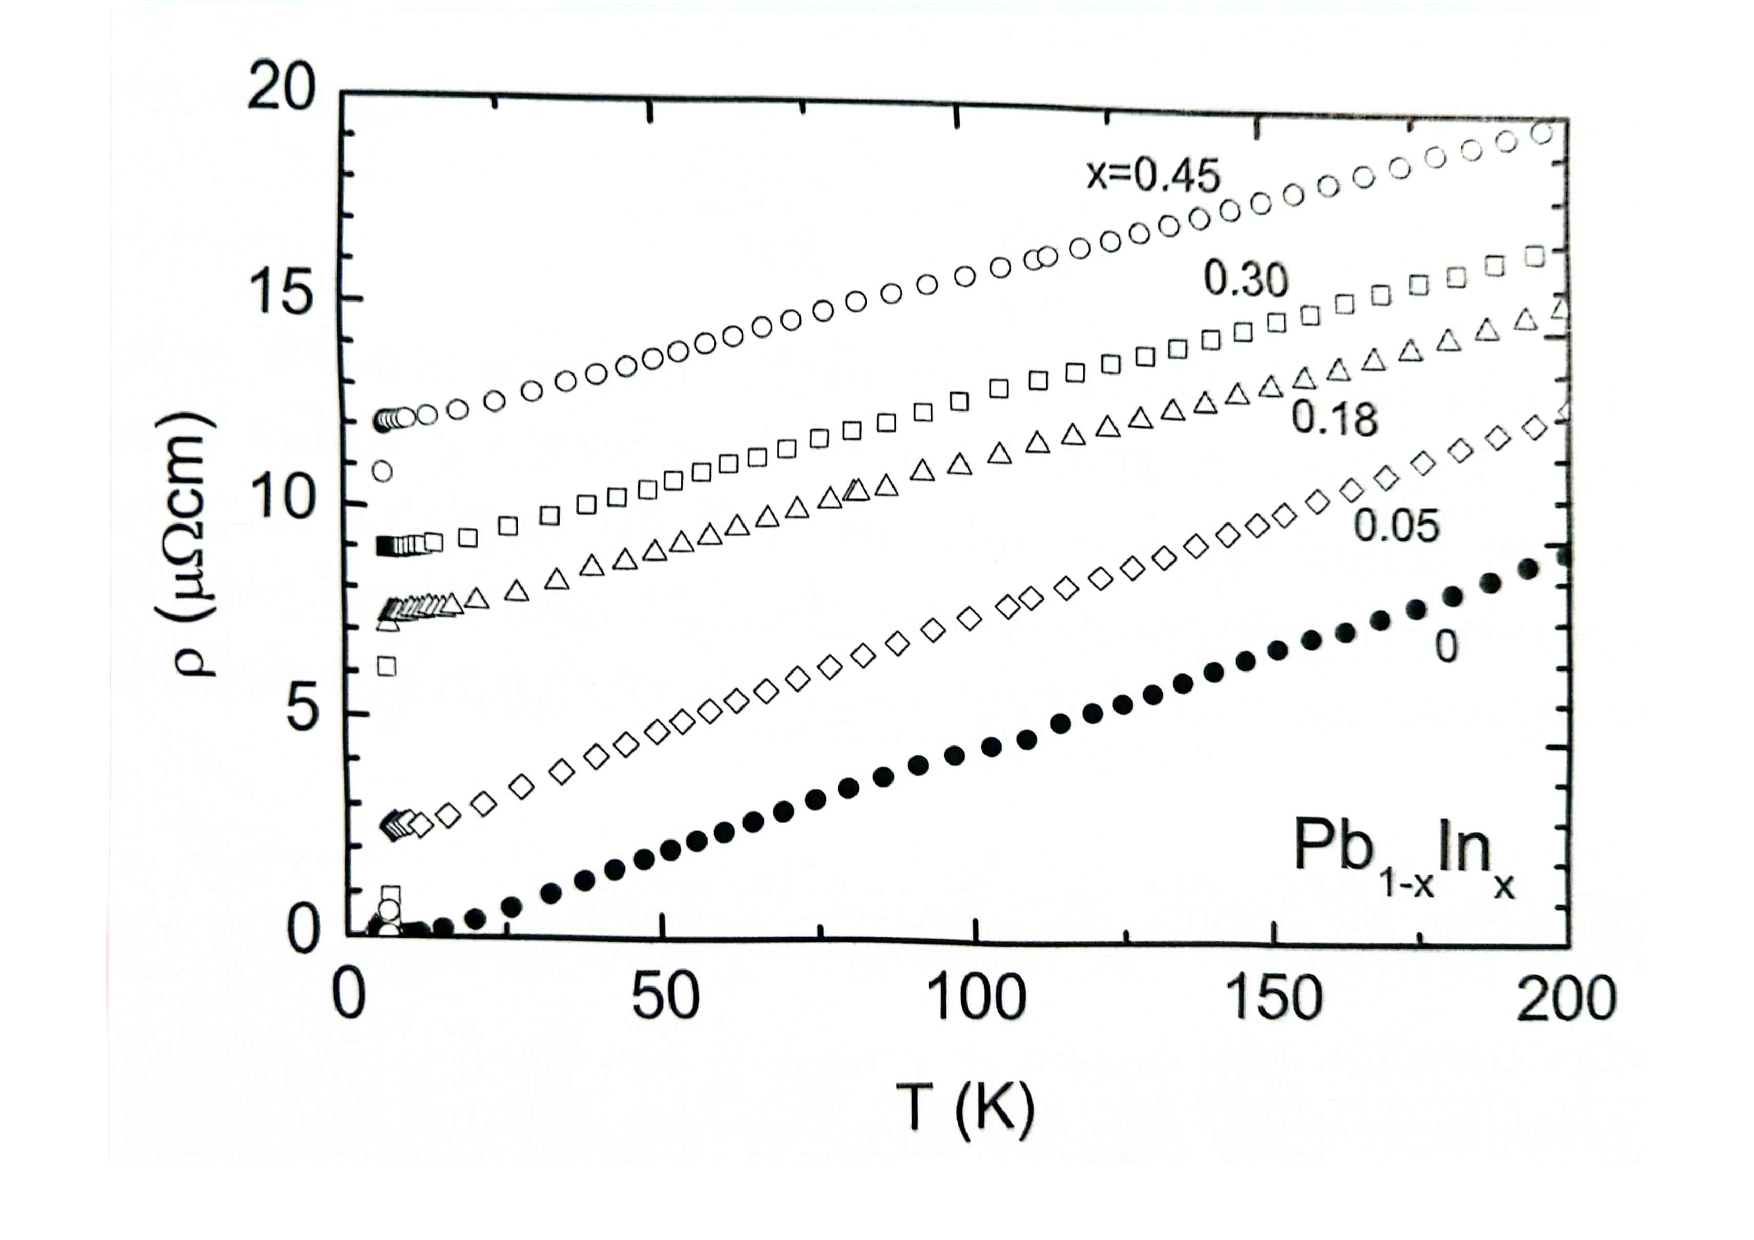
\includegraphics[scale=0.35]{Cuerpo/Ch_06/Fotos libro 6.pdf}
    \caption{Comprobación de la regla de Mathiessen con la resistividad de aleaciones de Pb-In. Al aumentar $x$ el desorden de la aleación y por tanto la contribución constante $\rho_{\text{def}}$ frente a $\rho_{\text{fon}} (T)$ que casi no cambia (nótese que la pendiente no varía). Es interesante que estas aleaciones son superconductores por debajo de $\sim 7$ K (veáse Capítulo \ref{Ch:11}).}
    \label{Fig:06-06}
\end{figure}  


\section{Conductivdad térmica electrónica}

A los electrones les es aplicable la expresión general $\kappa=\frac{1}{3}cv\ell$ donde $c$ es el calor específico electrónico, $v$ una velocidad característica del gas ($v\sim v_F$) y $\ell = v \tau$. Utilizando las ecuaciones (\ref{Ec:06-02-02}), (\ref{Ec:06-01-05}), (\ref{Ec:06-01-07}) y (\ref{Ec:06-01-08}) resulta

\begin{eqnarray}
	\kappa_{\text{el}} = \frac{\pi^2 n k_B^2 T_\tau}{3m}
\end{eqnarray}
su evolución con la temperatura es cualitativamente similar a la conductividad térmica reticular. En metales puros $\kappa_{el}$ es dominante a todas las temperaturas (uno o dos órdenes de magnitud mayor), aunque en metales impuros o aleaciones desordenadas puede competir con la contribución reticular. Observar qeu de nuevo no podmeos comparar $\kappa_{el}$ con el valor experimental porque desconocemos $\tau$

\section{Ley de Wiedmann-Franz}

Es un hecho notable que tanto $\sigma$ como $\kappa$ dependan linealmente del tiempo medio entre colisiones. Esto sugiere trabajar con la razón $L\equiv \kappa / \sigma T$, llamada \textit{número de Lorentz}. De nuestros resultados previos se obtiene fácilmente 

\begin{equation}
L=\frac{\pi^2 k_B^3}{3e^2} = \num{2.45e-8}
\end{equation}
de modo que $\kappa /\sigma T$ es una constante universal. Los resultados experimentales reprsentenativos mostrados en la tabla \ref{Tab:06-02} confirman excelentemente nuestra predicción, al menos a altas temperaturas. Hay que decir, sin embargo, que para $T\ll \theta_D$, $L_{\text{exp}}$ desciende apreciablemente; por ejemplo, para el Cu puro $L_{\text{exp}}(\unit{15 \kelvin}) \sim 0.1 L_{\text{teo}}$. La razón se atribuye a una posible difernecia entre tiempos de relajación térmico y eléctrico.

\begin{table}[h!] \centering
\begin{tabular}{ccc}
	Elemento & $L_{\text{exp}} (\unit{273 \kelvin})$ & $L_{\text{exp}} (\unit{373 \kelvin})$  \\
	& $10^8\unit{\watt \Omega / \kelvin^2}$ &  $10^8\unit{\watt \Omega / \kelvin^2}$ \\ \hline
	Ag & 2.31 & 2.37 \\
	Cu & 2.23 & 2.33 \\
	W  & 3.04 & 3.20 \\
	Zn & 2.31 & 2.33 \\
	Pt & 2.51 & 2.60
\end{tabular}	
\caption{Números de Lorentz experimentales para varios elementos.}
\label{Tab:06-02}
\end{table}

\section{Efecto Hall y magnetorresistividad}

En este aparatado se estudia la influencia sobre la conducción electrónica de un campo mangético externo. La configuración experimental típica (Hall 1879) se muestra la figura \ref{Fig:06-07}. La componente magnética de la fuerza de Lorentz produce una deflexión de las trayectorias electrónicas electrónicas que da lugar a una acumulación de carga en los bordes de la muestra. Asociado a ella aparece un campo eléctrico \textit{transversal}, $E_y$, que crece con la acumulación de carga hasta qeu contrarrestra la fuerza de Lorentz magnética y se establece un régimen estacionario.

\begin{figure}[h!] \centering
    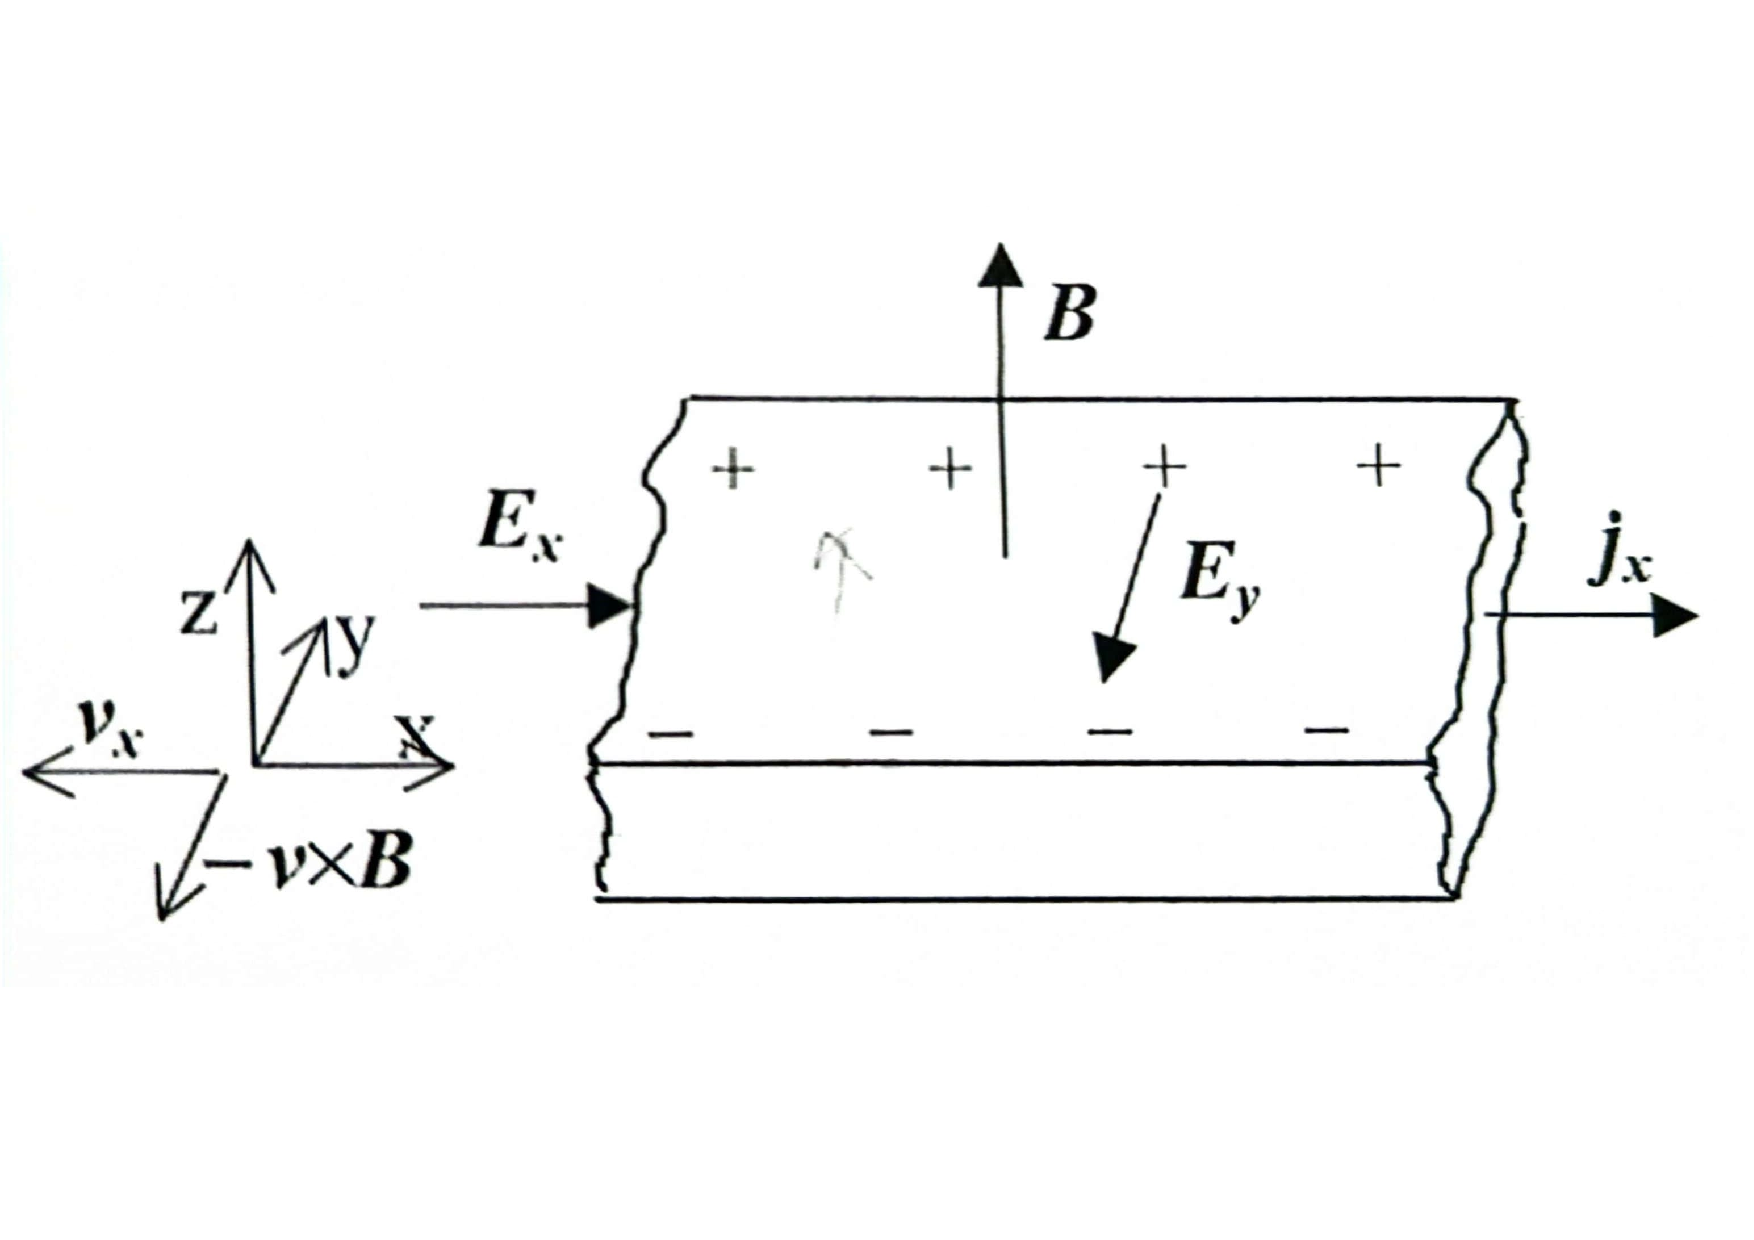
\includegraphics[scale=0.35]{Cuerpo/Ch_06/Fotos libro 7.pdf}
    \caption{Configuración experimental para comprobar el efecto Hall.}
    \label{Fig:06-07}
\end{figure}  

Las cantidades de interés son dos, ambas de fácil medida. La primera es la \textit{magnetorresistividad}

\begin{equation}
	\rho \equiv \frac{E_x}{\rho_x} \label{Ec:06-06-01}
\end{equation}
así llamada porque es de esperar que sea dependiente de $\Bn$. La segunda, que concierne al campo eléctrico transversal, se denomina \textit{coeficiente  Hall}

\begin{eqnarray}
	R_H \equiv \frac{R_y}{j_x B} \label{Ec:06-06-02}
\end{eqnarray}
Aplicando la ecuación dinámica (\ref{Ec:06-03-02}) en régimen estacionario y con $\fn (t) = q(\Encal + \vn \times \Bn)$ , se obtiene 

\begin{eqnarray}
	m \frac{\vn}{\tau} = q (\Encal + \vn \times \Bn)
\end{eqnarray}
y en componentes

\begin{equation}
\begin{split}
	v_x \  = \  & \ \frac{E_x q\tau}{m} - \omega_c \tau v_y \\
	v_y \  = \  & \ \frac{E_y q\tau}{m} + \omega_c \tau v_x \\
	v_z \  = \  & \ \frac{E_z q\tau}{m}  \label{Ec:06-06-04}
\end{split}
\end{equation}
en donde $\omega_c = eB/m$ es la llamada frecuencia ciclotrón. En la configuración experimental dada debemos hacer $v_y = 0$ pues no pueden haber corriente transversal neta. Utilizando que $\jn = nq\vn$ y sustituyendo  (\ref{Ec:06-06-04}) en (\ref{Ec:06-06-01}) y (\ref{Ec:06-06-02}) se llega fácilmente a 

\begin{eqnarray*}
	\rho =  \frac{m}{nq^2\tau}
\end{eqnarray*}
\begin{equation}
	R_H=\frac{1}{nq} \label{Ec:06-06-05}
\end{equation}

\begin{table}[h!] \centering
\begin{tabular}{ccc c ccc}
	Metal & Valencia & $R_H^{\text{exp}}/R_H^{\text{teo}}$ & & Metal & Valencia & $R_H^{\text{exp}}/R_H^{\text{teo}}$ \\ \cline{1-3} \cline{5-7} 
	Li & 1 & 1.25 & & Na & 1 & 0.83 \\
	K & 1 & 0.83 & & Rb & 1 & 1.0 \\
	Cs & 1 & 1.1 & & Cu & 1 & 0.67 \\
	Ag & 1 & 0.77 & & Au & 1 & 0.67 \\
	Be & 2 & -5 & & Mg & -2.5 \\
	In & 3 & -3.3 & & Al & 3 & -3.3 
\end{tabular}
\caption{Coeficiente Hall de algunos elementos (relativos al resultado de la teoría de e$^-$ libres).}
\label{Tab:06-03}
\end{table}

En conclusión, nuestro modelo predice que 

\begin{enumerate}
	\item La magnetorresistividad es independiente del campo magnético externo $\rho(\Bn)=\rho(0)$.
	\item $R_H<0$ (dado que $q=-e$), dependiendo su magnitud sólo de la concetración electrónica. 
\end{enumerate}
Experimentalmente, la magnetorresistividad presenta gran variedad de comportamientos. Para algunos metales la dependencia es débil; para otrosm satura a un valor constante para altos valores de $B$, pero para ciertas orientanciones crece sin límite (volveremos a ello en el Capítulo \ref{Ch:08}). En cuanto al coeficiente Hall, el datos experimentales es bueno para los metales alcalinos, relativamente aceptable para los metales nobles e inaceptables para otros. En particular resulta inexplicable el signo positivo de $R_H^{\text{exp}}$ a menos que aceptáramos que los portadores de carga fueran positivos, lo cual a su vez es incompatible con un modelo de elctrones libres. En general, además $R_H = R_H (\Bn)$, aunque (\ref{Ec:06-06-05}) puede aún ser válida en el límite de campos magnéticos altos. Estas discrepancias se resuelven dentro de la Teoría de Bandas (Capítulo \ref{Ch:07}), que incluye la interacción de los electrones con el potencial periódico que producen los iones de la red.

\section{Conductividad AC y propiedades ópticas}

Se estudia en apartado la predicción del modelo de electrones libres para algunas de las magntiudes ópticas básicas como la reflectividad y la atenuación. Supóngase un campo electromagnético de frecuencia $\omega$ aplicado sobre el metal. Despreciando el efecto del campo magnético asociado y prescindiendo del carácter vectorial, la ecuación dinámica (\ref{Ec:06-03-02}), puede expresarse como $m\dot{v}=-mv/\tau-eE_0e^{-i\omega t}$. Probando para la velocidad media de portadores una solución de la forma $v=v_0 e^{i\omega t}$ (donde $v_0$ puede ser complejo para tener en cuenta posibles desfases) resulta $v=-e\tau E / m(1-i\omega\tau)$. Usando ahora $j=-nev$, se obtiene directamente $j=\sigma(\omega)E$ donde 
 
\begin{eqnarray}
	\sigma (\omega) = \frac{\sigma(0)}{1-i \omega \tau} \label{Ec:06-07-01}
\end{eqnarray}
Aquí $\sigma (0) = ne^2 \tau/m$ es la conductividad eléctrica para $\omega=0$, es decir, DC. Una primera consecuencia de (\ref{Ec:06-07-01}) es que cuando $\omega \tau \ll 1$, $\sigma (\omega) \approx \sigma (0)$, la corriente oscila a la misma frecuencia que $\Encal$, gracias a las colisiones, y el comportamiento es puramente resistivo. Sin embargo, cuando $\omega \tau \gg 1$ las colisiones no son lo suficientemente frecuentes para frenar la inercia de los electrones y éstos se retrasan con respecto a $\Encal$, diminuyendo la absorción de energía.

Aunque $\sigma (\omega)$ contiene en principio toda la respuesta del gas, es más conveniente utilizar la \textit{formulación óptica}, que consiste en usar permitividad eléctrica relativa $\varepsilon(\omega)$. Recuérdese que las ecuaciones de Maxwell conducen a la siguiente relación entre $\varepsilon (\omega)$ y $\sigma (\omega)$ 
 
\begin{eqnarray}
	\varepsilon (\omega) = 1 + \frac{i \sigma(\omega)}{\varepsilon_0 \omega} \label{Ec:06-07-02}
\end{eqnarray}
Al sustituir (\ref{Ec:06-07-01}) en (\ref{Ec:06-07-02}) se obtiene 

\begin{eqnarray}
	\varepsilon(\omega) = 1 + \frac{i \sigma_0 / \varepsilon_0 \omega}{1-i\omega \tau} \label{Ec:06-07-03}
\end{eqnarray}
Dos casos límtie de (\ref{Ec:06-07-03}) son especialmente interesantes:

\begin{itemize}
	\item \textbf{Frecuencia bajas:} $\omega \tau \ll 1$ y $\omega \ll \sigma / \varepsilon_0$. Por ejemplo, en el cobre esto se cumple para $\omega/2\pi\ll 10^{12} \ \unit{\Hz}$ ($\lambda = 0.3\unit{\mm}$), que está en la frotera entre ondas muy cortas radio y el infrarrojo. En este límite (\ref{Ec:06-07-03}) queda 
	\begin{eqnarray}
		\varepsilon(\omega) = \frac{i\sigma_0}{\varepsilon_0 \omega}
	\end{eqnarray}
	Introduciendo el índice de refracción $n=\sqrt{\varepsilon(\omega)}=n_1 + i n_2$, y teniendo en cuenta $\sqrt{i}=(1+i)/\sqrt{2}$, resulta
	\begin{eqnarray}
		n = \sqrt{\frac{\sigma_0}{2\varepsilon_0\sigma}} (1+i) \label{Ec:06-07-05}
	\end{eqnarray}
	Al haber parte imaginaria habrá \textit{atenuación}: la amplitud del campo eléctrico se atenúe como $E\propto e^{ikx} \propto e^{\omega n_2 x/c} = e^{-x/2\delta}$ (se ha utilizado la relación de dispersión general de las ondas electromangéticas $\omega = ck /n$). La onda recorre una distnacia $\delta$ antes de atenuarse, llamada \textit{profundidad de penetración}, que viene dada por 
	\begin{eqnarray}
		\delta = \sqrt{\frac{2\varepsilon_0 c^2}{\sigma_0 \omega}}
	\end{eqnarray}
	Por ejemplo para el cobre y con $\omega/2\pi \approx 10^{10} \unit{\Hz}$ (microondas $\lambda=3\unit{\cm}$) $\delta$ es tan sólo de unos $10 \ \unit{\um}$. En cuanto a la reflectividad 

	\begin{eqnarray}
		r = \left| \frac{n-1}{n+1} \right|^2 = \frac{(n_1-1)^2 + n_2^2}{(n_1+1)^2+n_2^2} \label{Ec:06-07-07}
	\end{eqnarray}
	Como, por (\ref{Ec:06-07-05}), $n_1 = n_2 = \sqrt{\sigma / 2\varepsilon_0 \omega} \gg 1$ (límite de bajas frecuenias), se tiene que $r\approx 1$, o sea, la reflectividad tiende al 100\%. De hecho es una regla general que cuanto más abosbe un material tanto más refleja en la superficie.

	\item \textbf{Frecuencias altas:} $\omega \tau \ll 1$. En este límite (\ref{Ec:06-07-03}) se aproxima por 
	\begin{eqnarray}
	\varepsilon (\omega) \approx 1 - \frac{\sigma_0 /\varepsilon_0 \tau}{\omega^2} = 1 - \frac{\omega_p^2}{\omega^2}
	\end{eqnarray}
	donde $\omega_p^2 = \sigma_0 / \varepsilon_0 \tau = ne^2 / \varepsilon_0 m$ se denomina \textit{frecuencia de plasma}. Se puede comprobar que $\omega_p$ corresponde a la frecuencia caractrística de oscilaciones longitudianles de la densidad de densidad del gas de electrones, cuyo \textit{cuanto} se denomina \textit{plasmón}. Estos modos de vibración electrónicas son muy energéticos corresponde al U.V. Para $\omega < \omega_p$, $\varepsilon(\omega)<0$, $n\approx n_2$ y existe atenuación. Asimismo, se ve en (\ref{Ec:06-07-07}) que $r \rightarrow 1$ al tender $n_1 \rightarrow 0$. Sin embargo, para $\omega > \omega_p$,$\varepsilon(\omega)$ es real, $n_2=0$ y el metal se hace \textit{transparente}. Esta transparenecia debe ocurrir en el U.V. Para algunos metales, como los alcalinos, esto se verifica bien. En general, las propiedes óptica de los metales son menos simples de los que predica el modelo de electrones libres y, de nuevo, la estructura de badndas es de referencia obligdaa para su explicación.
\end{itemize}